\documentclass[a4paper,12pt]{article}
\usepackage{tabularx} 
\usepackage{graphicx} 
\usepackage[margin=1in,letterpaper]{geometry} 
\usepackage{indentfirst}

\begin{document}
\title{Introduction to Artificial Intelligence\\
Assignment 1 report}
\author{Elina Akimchenkova, BS21-07 Student,\\
e.akimchenkova@innopolis.university}
\date{Fall semester 2022}
\maketitle

\section{Assumption}
The assignment's description is unclear, and in order to complete it, you must rely on a number of assumptions.
\begin{enumerate}
    \item Agent can not go out of bounds of field
    \item Agent ALWAYS present on cell (0,0), even if there is no in the input file
    \item Cost of moving horizontal, vertical and diagonal is 1
    \item There are two ways to solve the problem:
    \begin{enumerate}
        \item Direct way to Dead’s Men Chest
        \item Jack has to be able to slay the Kraken on his route from Tortuga to Dead's Men Chest Island, hence he must travel through Tortuga Island
    \end{enumerate}
\end{enumerate}

\section{PEAS description of Jack Sparrow}
\begin{enumerate}
    \item \textbf{Performance measure -} finding the shortest path to the Dead Man’s Chest on the Island of the Cross
    \item \textbf{Environment -} Ocean near the Island of the Cross (\(9\times 9\) matrix)
    \item \textbf{Actuators -} moving, capturing Tortuga, and slaying Kraken
    \item \textbf{Sensors -} spyglass (perception zone that depends on scenario)
\end{enumerate}
\subsection{Properties of the environment}
\begin{enumerate}
    \item \textbf{Partially Observable -} Jack Sparrow can see only in his perception zone
    \item \textbf{Single Agent -} On the map, only Jack Sparrow may move; all other objects are stationary
    \item \textbf{Sequential -} Future actions are affected by the present choice, thus if Jack kills the Kraken, he can move in its location without suffering harm
    \item \textbf{Dynamic -} By slaying Kraken, Agent can alter the environment
    \item \textbf{Discrete -} Jack Sparrow moves from cell to cell in deliberate movements
    \item \textbf{Known -} Agent is familiar with the locations of Tortuga Island and Dead Man's Chest since he carries a compass.
\end{enumerate}

\section{Search algorithm description}
\subsection{BackTracking algorithm}
The backtracking search tries all of possible paths and looking for the shortest with DFS. It use a 2D array of visited cells with the shortest path to them. When the algorithm starts to explore the possibilities, the recursion function is used to check whether the suggested solution satisfies the constraints. It will continue looking if it does. If not, the branch is deleted and the algorithm goes back to the previous level.

But I did make a optimizations to it. The goal of optimization is to maintain track of already discovered pathways and reject backtracking branches that lead to longer paths than those that have already been discovered. 

\subsection{AStar algorithm}
A search algorithm known as AStar algorithm looks for the shortest path between the starting cell and the final cell. The AStar algorithm uses three parameters:
\begin{enumerate}
    \item \textbf{g} - the sum of all the cells that have been visited since leaving the first cell.
    \item \textbf{h} - heuristic value, it is the estimated cost of moving from the current cell to the final cell
    \item \textbf{f} - the sum of g and h
\end{enumerate}
The f-value is a factor that the algorithm considers when coming to a decision. The algorithm proceeds to the cell with the least f-value. This procedure keeps on until the algorithm achieves its objective.

\section{Algorithms comparison}
\subsection{Testing algorithms on several maps}
There were generated 1000 several maps (for statistical analysis of each algorithm). To generate the map, a function was used, which creates the random coordinates for each character (from range [0, 9)), taking into account all limitations (coincidence of the position of the Kraken or Davy Jones and the Dead Man's Chest etc.).

\subsection{Maps with no solutions}
Both algorithms can solve absolutely \textbf{ALL} maps, but there are a number of maps that cannot be won, since there is no path leading to the Dead Man's Chest.
\subsubsection{Legend}
\begin{enumerate}
    \item JS – Jack Sparrow
    \item T – Tortuga
    \item DMC – Dead’s Men Chest 
    \item K – Kraken
    \item R – Rock
    \item DJ – Davy Jones
\end{enumerate}

\subsection{Graphical representation of maps}
\begin{figure}[h]
         \centering
         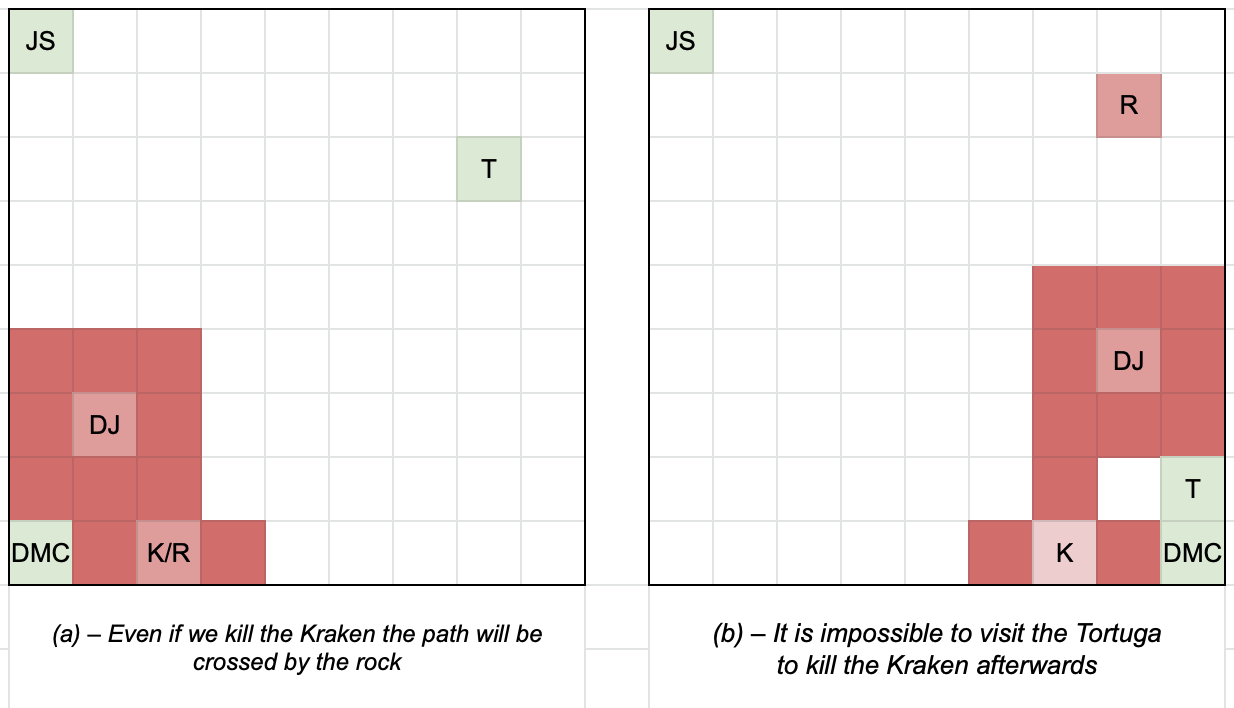
\includegraphics[width = 0.8\textwidth]{images/mapsab.png}
\end{figure}

\begin{figure}[h]
         \centering
         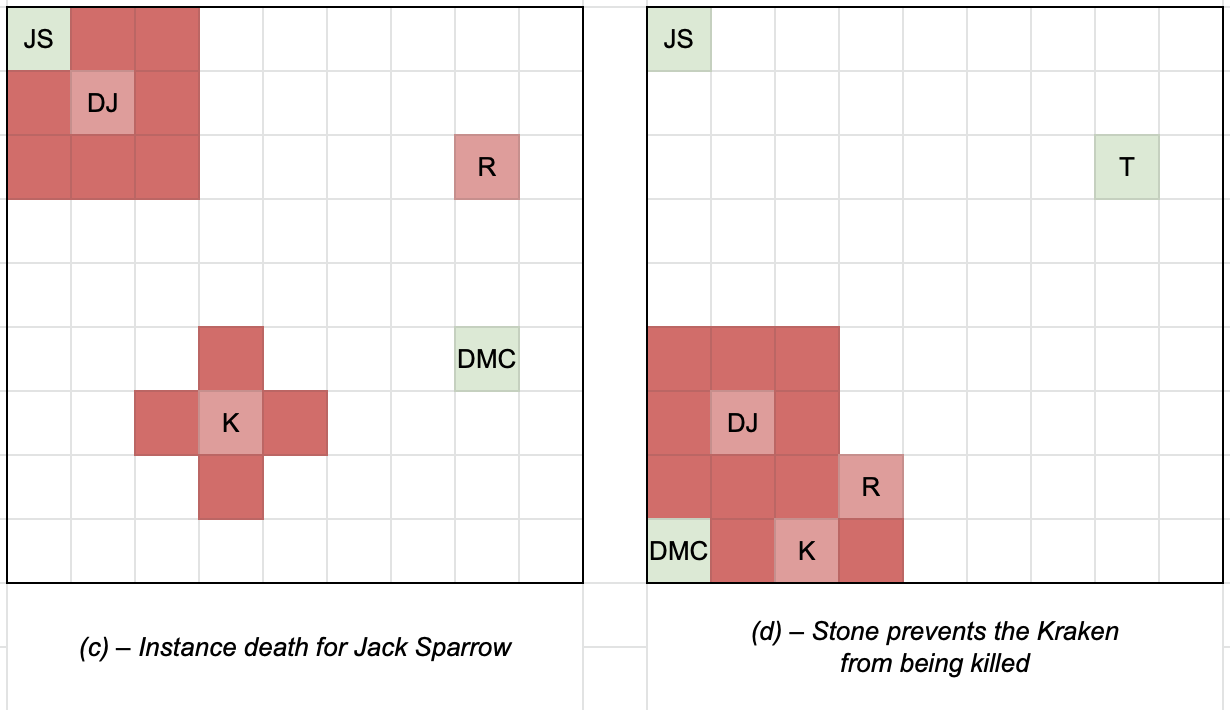
\includegraphics[width = 0.8\textwidth]{images/mapcd.png}
\end{figure}

\newpage
\subsection{Statistical Analysis}
\begin{center}
\begin{tabular}{ |p{5cm}|p{2.5cm}|p{2.5cm}|p{2.5cm}|p{2.5cm}| }
    \hline
    & Backtracking&AStar&Backtracking&AStar\\
    \hline
    Scenario number&\multicolumn{2}{|c|}{1} & \multicolumn{2}{|c|}{2}\\
    \hline
    Mean of time for execution (ms) & 3.289 & 0.034 & 6.756 & 0.038\\
    Mode of time for execution (ms) & 3.35  & 0.02 &6.35& 0.02\\
    Median of time for execution (ms)& 3.239 & 0.025 &6.597& 0.029\\
    Standard deviation of time for execution (ms) & 3.467 & 0.096 &7.395& 0.071\\
    \hline
    Number of wins & \multicolumn{4}{|c|}{938} \\
    Number of loses & \multicolumn{4}{|c|}{62}  \\
    Percentage of wins & \multicolumn{4}{|c|}{93.8\%} \\
    Percentage of loses & \multicolumn{4}{|c|}{6.2\%} \\
    \hline
\end{tabular}
\end{center}
The table shows that in both cases, AStar solves the issue faster than Backtracking, although algorithms are the same while trying to discover a path (if one algorithm finds a path, the second will find it too). 
It's also noteworthy that the first scenario runs the algorithm faster than the second one if you compare how quickly it operates in the various conditions.
\section{Source Code}
Java source code files, together with report are available
on my Github repository, the link: \href{https://github.com/akmchnkv/Compass-and-Pirates}.\\
\end{document}

